\documentclass[9pt, aspectratio=169]{beamer}

% Theme settings
\usetheme{Copenhagen}
\usecolortheme{seahorse}
\usefonttheme{serif}

\setbeamerfont{frametitle}{size=\fontsize{14}{16}\selectfont}
\setbeamersize{text margin left=0.5cm, text margin right=0.5cm}
% Encoding & Fonts
\usepackage[T1]{fontenc}
\usepackage[utf8]{inputenc}
\usepackage{graphicx}
\usepackage{caption}
\usepackage[inkscapeformat=png]{svg}
\usepackage{amsmath, amsfonts, amssymb}
\usepackage{multicol}
\usepackage{ragged2e}
\usepackage[absolute,overlay]{textpos}
\usepackage{changepage}
\usepackage{hyperref}
\hypersetup{hidelinks}
\usepackage{tikz}
\usetikzlibrary{positioning}
\usepackage{fontawesome5} % For social media icons

% Bibliography
\usepackage[style=authoryear]{biblatex}
\addbibresource{biblio.bib}

\renewcommand*{\nameyeardelim}{\addcomma\space}
\newcommand{\customcite}[1]{\textcolor{blue}{\footnotesize\parencite{#1}}}
\newcommand{\customcites}[1]{\textcolor{blue}{\footnotesize\parencites{#1}}}
\AtEveryCite{\renewcommand{\bibsetup}{\nopagenumbers}}

% Customize bibliography format
\DeclareFieldFormat{title}{\mkbibemph{#1}} 
\DeclareFieldFormat[article]{volume}{\textbf{#1}}
\DeclareFieldFormat[article]{number}{\mkbibparens{#1}} 
\DeclareFieldFormat{pages}{#1} 
\DeclareFieldFormat{doi}{\newline\mkbibacro{DOI}: \href{https://doi.org/#1}{#1}} 
\DeclareFieldFormat{url}{\newline\mkbibacro{URL}: \href{#1}{#1}}

\renewbibmacro{in:}{}
\renewcommand*{\bibfont}{\footnotesize} % Smaller font for bibliography

% Remove hyperlinks to bibliography slide
\setbeamertemplate{bibliography item}{}
\setbeamertemplate{frametitle continuation}{}
\setbeamertemplate{headline}{}
\setbeamertemplate{footline}{}
\setbeamertemplate{bibliography item}{}

% Custom Footer
\setbeamertemplate{footline}{
    \leavevmode%
    \hbox{%
      \begin{beamercolorbox}[wd=.45\paperwidth,ht=2.25ex,dp=1ex,center]{author in head/foot}%
        \usebeamerfont{author in head/foot}\shortauthor
      \end{beamercolorbox}%
      \begin{beamercolorbox}[wd=.45\paperwidth,ht=2.25ex,dp=1ex,center]{title in head/foot}%
        \usebeamerfont{title in head/foot}\shorttitle
      \end{beamercolorbox}%
      \begin{beamercolorbox}[wd=.1\paperwidth,ht=2.25ex,dp=1ex,center]{date in head/foot}%
        {\fontsize{6}{7.2}\selectfont \insertframenumber{}/19}
      \end{beamercolorbox}}%
    \vskip0pt
}

 
 % Remove navigation symbols
 \setbeamertemplate{navigation symbols}{}

% Short Title and Author for Footer
\newcommand{\shorttitle}{PhD Project Colloquium}
\newcommand{\shortauthor}{Stefano Sangiovanni}

%% Title Page
\date{\footnotesize NASP-POLS PhD Project Colloquium \\ April 22, 2025}

\title{\textbf{The Strategic Balance Between Positional and \\ Valence Issues in Party Competition}}

\author{
    \large\textbf{Stefano Sangiovanni} \\[0.3cm]
     Supervisors: Andrea Ceron\textsuperscript{1}, Giovanna M. Invernizzi\textsuperscript{2}
}

\institute{
    \footnotesize
    \textsuperscript{1} Department of Social and Political Sciences, University of Milan \\
    \textsuperscript{2} Department of Social and Political Sciences, Bocconi University
}


\begin{document}

\begin{frame}[plain]
    \titlepage
\end{frame}

\begin{frame}{Structure of the Presentation}
    \setcounter{framenumber}{1}
    \begin{enumerate}
        \item Introduction and Theoretical Background \vspace{0.4cm}
        \item Experimental Designs \vspace{0.4cm}
        \begin{itemize}
            \item Conjoint Experiment \vspace{0.2cm}
            \item Audio-Based Survey Experiment
        \end{itemize}\vspace{0.4cm}
        \item Overview of the Other Papers \vspace{0.4cm}
        \item Conclusions and Next Steps \vspace{0.4cm}
    \end{enumerate}
    \end{frame}

\begin{frame}{Overview of the PhD Project}
    \textbf{Valence theory:} voters are influenced not only by policy positions, but also by concepts on which all voters hold near-identical preferences \customcites{stokes1992valence, clark2009valence} \vspace{0.2cm}
        \begin{itemize}
            \item \textbf{Policy-based:} perceived competence on universally valued goals \customcites{groseclose2001model, jacoby2009public, clark2009valence} \vspace{0.2cm}
            \item \textbf{Character-based:} traits like honesty, competence, charisma, and unity \customcites{clark2009valence, adams2001theory}
        \end{itemize}
\vspace{0.3cm}
\textbf{Research Focus:} \vspace{0.1cm}
\begin{itemize}
    \item How political parties strategically use \textbf{valence appeals} to shape voter perceptions and structure party competition across different arenas (e.g., parliamentary debates, electoral campaigns) \vspace{0.2cm}
    \item How parties navigate the trade-off between \textbf{positional} and \textbf{valence-based} strategies \vspace{0.2cm}
    \item How \textbf{negative valence shocks}, such as political scandals or negative news about the state of the economy, shape voters’ evaluations of politicians and parties
\end{itemize}

\end{frame}

% \begin{frame}{Introduction and Theoretical Background}
%     \begin{itemize}
%         \item \textbf{Valence theory:} Voters are influenced not only by policy positions, but also by concepts on which all voters hold near-identical preferences \customcites{stokes1992valence, clark2009valence} \vspace{0.2cm}
%         \begin{itemize}
%             \item \textbf{Policy-based:} perceived competence on universally valued goals \customcites{groseclose2001model, jacoby2009public, clark2009valence} \vspace{0.2cm}
%             \item \textbf{Character-based:} traits like honesty, competence, charisma, and unity \customcites{clark2009valence, adams2001theory}
%         \end{itemize}
%         \vspace{0.4cm}
        
%         \item \textbf{Research Focus:} \vspace{0.1cm}
%         \begin{itemize}
%             \item How parties strategically use valence appeals to shape voter perceptions and structure party competition in different contexts (parliamentary debates, electoral campaign) \vspace{0.2cm}
%             \item How they navigate the trade-off between \textbf{positional} and \textbf{valence-based} appeals \customcites{stokes1992valence, clark2009valence}\vspace{0.2cm}
%             \item How \textbf{negative valence shocks}, such as political scandals, affect voter perceptions of politicians
%         \end{itemize}
%     \end{itemize}
% \end{frame}


\begin{frame}{Structure of the Dissertation - 3 Interconnected Papers}
    \textbf{Political Scandals and Voter Evaluations}  \vspace{0.2cm}
    \begin{itemize}
        \item Examines the effects of political scandals on voter perceptions using two experiments: \vspace{0.1cm}
        \begin{itemize}
            \item Conjoint experiment\vspace{0.1cm}
            \item Audio-based survey experiment
        \end{itemize}
    \end{itemize}
\vspace{0.3cm}
    \textbf{Electoral Campaigns and Valence}  \vspace{0.2cm}
    \begin{itemize}
        \item Investigates how parties’ valence statements during campaigns affects polling support
    \end{itemize}
    \vspace{0.3cm}
    
    \textbf{Economic Performance and Strategic Valence}  \vspace{0.2cm}
    \begin{itemize}
        \item Explores how governing and opposition parties adjust valence strategies in response to economic indicators
    \end{itemize}
\end{frame}

%The second paper examines the effect of positive economic indicators on valence emphasis, investigating how governing parties leverage favorable economic performance to enhance their competence and leadership image, while opposition parties may shift focus to positional economic issues, such as inequality and redistribution.

\begin{frame} %Trump in 2016
    \begin{figure}
        \centering
        \includegraphics[width=\linewidth]{images/Trump1.png}
        \label{fig:trump1}
    \end{figure}
        \begin{figure}
        \centering
        \includegraphics[width=0.7\linewidth]{images/Trump2.jpg}
        \label{fig:trump2}
    \end{figure}
\end{frame}

\begin{frame}{Political Scandals and Valence Theory}
    \begin{itemize}
        \item Political scandals involve \textbf{norm-breaking behavior} that violates societal norms, moral codes, or values \customcites{genovese_2010, Thompson_2013} \vspace{0.3cm}
        \item Allegations of illegal, unethical, or immoral conduct directed at politicians or institutions \customcite{Rottinghaus_2023}, they attract public scrutiny and attention \customcites{Thompson_2013, Marion_2010}\vspace{0.2cm}
        \item If scandals are perceived as \textbf{negative valence information}, then voters should negatively evaluate involved politicians \customcites{doherty2014does, Rottinghaus_2023} \vspace{0.3cm}
        \item Some studies find that scandals have negative political consequences even in polarized contexts \customcites{darr2019collision, wolsky2022scandal}, while others suggest minimal impact on politicians' careers and electoral behavior \customcites{funck2021partisanship, Lee_2023}
    \end{itemize}
\end{frame}

% \begin{frame}{Valence Theory and Political Scandals}
%     \begin{itemize}
%     %its quite established in the literature that
%     \item \textbf{Valence issues} are key factors influencing voter behaviour alongside traditional left-right distinctions and policy positions \customcite{groseclose2001model, jacoby2009public, clark2009valence} \vspace{0.3cm}
%     \item Valence dimensions refer to “character-based values” like honesty, competence, charisma, likability and unity \customcites{clark2009valence, adams2001theory} \vspace{0.3cm}
%     \item Political scandals, exposing misconduct or corruption, shape perceptions of candidate integrity and competence \customcites{doherty2014does, Rottinghaus_2023} \vspace{0.3cm}
%     \item If scandals are perceived as \textbf{negative valence information}, then voters should negatively evaluate involved politicians \customcites{doherty2014does, Rottinghaus_2023} \vspace{0.3cm}
%     \item Voters should appreciate politicians who are not involved in any scandals and should judge those that are involved
%     \end{itemize}
% \end{frame}

%%% PAPER TRE EXPERIMENTS

% \begin{frame}{Political Scandals: A Definition}
%     \begin{itemize}
%         \item Characterized by \textbf{norm-breaking behavior} deviating from societal norms, moral codes, or values \customcites{genovese_2010, Thompson_2013} \vspace{0.3cm}
%         \item Allegations of illegal, unethical, or immoral conduct directed at politicians or institutions \customcite{Rottinghaus_2023}, they attract public scrutiny and attention \customcites{Thompson_2013, Marion_2010}\vspace{0.2cm}
%         \begin{itemize}
%         \item \textbf{Financial Scandal}: personal financial gain from actions (e.g., corruption, bribery, tax evasion) 
%         \item \textbf{Personal Scandal}: immoral, illegal or unethical personal behavior (e.g., drug use, adultery, sexual allegations, cheating on CV) \vspace{0.3cm}
%         \end{itemize}
%         \item Some studies find that scandals have negative political consequences even in polarized contexts \customcites{darr2019collision, wolsky2022scandal}, while others suggest minimal impact on politicians' careers and electoral behavior \customcites{funck2021partisanship, Lee_2023}
%     \end{itemize}
% \end{frame}
%  Lee_2023
%         \item Scandals often expose negative portrayals affecting politicians' integrity and trust with constituents\vspace{0.3cm}
%         \item Different types of scandals may elicit varied reactions and meanings among voters\vspace{0.3cm}


% how voters process valence-related information

% when individuals and politicians share similar values, particularly co-partisanship or ideological alignment, the consequences and the magnitude of scandals may differ. Could a high level of partisanship and ideological polarization diminish the effects of a political scandal? If so, do all types of scandals have the same consequences? 


%%%%%% Research Questions

\begin{frame}{Research Design: Two Complementary Experiments}

\begin{block}{Main Research Question}  
\centering How does different types of \textbf{political scandals} shape voter evaluations of political candidates? 
\end{block}
\vspace{0.3cm}

\textbf{Experiment 1: Conjoint Design} \customcite{hainmueller2014}  
\begin{itemize}
    \item How do voters weigh different political scandals relative to other candidate attributes, such as party affiliation, policy positions, and positive valence?
    \item Do shared values (co-partisanship, ideological alignment) moderate the impact of political scandals on voter evaluations?
\end{itemize}
\vspace{0.2cm}
\textbf{Experiment 2: Audio-Based Survey Experiment}  
\begin{itemize}
    \item How does the tone and rhetorical delivery of a scandal accusation (calm vs. aggressive) influence voter perceptions of the accused politician?
    \item Do policy positions and ideological alignment condition the effect of scandal accusations on voter attitudes?
\end{itemize} 
\end{frame}

%%%%%%%%%%%%% Conjoint Experiment

\begin{frame}{The Conjoint Experiment}
    \begin{itemize}
        %\item Randomized conjoint design (with constrained randomization for valence attributes) \customcite{hainmueller2014} \vspace{0.2cm}
        \item Present \textbf{detailed-rich fictional scenario} where two candidates compete in an actual election \customcite{Galasso} \vspace{0.3cm}
        \item Participants will express a \textbf{preference between two politicians} with differing characteristics across various attributes \vspace{0.3cm}
        \item Each respondent completes \textbf{3 tasks}, each time choosing between \textbf{2 candidates} and indicating their preferred choice \vspace{0.3cm}
        \item \textbf{Sample:} 2,000 respondents per country (USA, UK) recruited via a survey company \vspace{0.3cm}
        \item \textbf{Power Analysis:} Our sample size allows us to detect a 0.04 effect for an attribute with 5 levels with 0.84 statistical power \customcite{lukac_stefanelli_2020}
    \end{itemize}
\end{frame}


%add several elements to provide a detailed picture of the politician, including personal background info.. maybe one scandal matters more (or less) when linked with some individual traits

% \begin{frame}{Experimental Design: Attributes and Levels}
%     \begin{itemize}
%         \item Candidate's traits: Gender, Party Affiliation \vspace{0.3cm}
%         \item Include real and relevant policy issues as attributes to immerse participants in a real-world context \customcite{morton2011electoral} \vspace{0.2cm}
% \begin{itemize}
%     \item e.g. Immigration, Green policies, Education, Taxation, EU integration \vspace{0.3cm}
% \end{itemize}
%         \item Focus on Financial and Personal scandals 
%         \customcite{Rottinghaus_2023} \vspace{0.3cm}
%         \item Use neutral categories for better interpretation of AMCEs \customcite{BansakEtAl2022} \vspace{0.3cm}
% % average marginal component effects
% \item Present candidate profiles in a "short bio" format for clarity and realism
%     \end{itemize}
% \end{frame}

\begin{frame}{Experimental Design: Profile Attributes}
\begin{itemize}
    \item \textbf{General Attributes:} Gender, Party Affiliation, Incumbency Status, Position on Immigration, Position on Economic Policies
\end{itemize}
\vspace{0.3cm}
\begin{table}[!h]
\centering
\resizebox{\textwidth}{!}{%
\begin{tabular}{|c|c|}
\hline
\textbf{Attributes}                 & \textbf{Levels}                                                                                                  \\ \hline
\textbf{Political Scandal} &  \begin{tabular}[c]{@{}c@{}}No scandal \\[2.0pt] Investigated for unwanted sexual conduct towards staff members \\[2.0pt] Falsification of credentials on curriculum vitae \\[2pt] Investigated for corruption \\[2pt] Participated in a violent anti-government protest while underage

 \end{tabular} \\ \hline
\textbf{Positive Valence} &  \begin{tabular}[c]{@{}c@{}}No positive valence \\[2.0pt] Had 95\% of campaign statements certified as accurate by an independent fact checker \\[2pt] Led public-private partnership preventing layoffs during local economic downturn \\[2pt] Successfully rallied party support for innovative policy agenda, turning initial 30\% backing into 90\% consensus \\[2pt] Voted with party positions on 93\% of legislative votes
 \end{tabular} \\ \hline
\end{tabular}%
}
\end{table}
\end{frame}



% we will use the Average Marginal Component Effect (AMCE; Hainmueller et al., 2014), which is the oldest and most used estimator for conjoint experiments. Yet, recent criticisms of this estimator are leading scholars to prefer marginal means (MM; see Baldassarri & De Jong, 2023; Casiraghi et al., 2023) which do not express the effects in terms of a reference category. Conveniently, both these estimators and subsequent visualizations have been implemented in the R package cjregg (Leeper, 2018). 

% Exploratory analyses regarding the interaction between profile attributes (ACIEs: Average Component Interaction Effects) and between attributes of the respondents and the profiles (subgroup analyzes) will additionally be run.

%\item  the degree to which a given value of a conjoint profile feature increases or decreases respondents’ support for the overall profile relative to a baseline, averaging across all respondents and all other profile features. 
 
% without going too much into details
% Average component interaction effect
% Average marginal components effect


%%%%%%%%%%%%%%%%%%%%%% Audio Experiment :D 

\begin{frame}{Audio Experiment}
\begin{itemize}

\item Investigate how the \textbf{tone of delivery} influences the effectiveness of valence attacks \customcites{Tigue2012, Gerstle2019, Kulz2023} \vspace{0.3cm}

\item Utilize open-source multi-voice \textbf{TTS technology} to simulate realistic political debates \vspace{0.3cm}

\item \textbf{Sample:} 2,000 respondents per country (USA, UK) recruited via a survey
company \vspace{0.3cm}

\item Participants will be randomly assigned to listen to one debate or read the text version. At the end of the experiment, respondents will indicate their preferred candidate \vspace{0.3cm}
%This design tests the impact of hearing the debate versus reading the text on participants' candidate preference. 
\item \textbf{Debate Structure (Approx. 2 minutes):} \vspace{0.2cm}
\begin{itemize}
\item An anchor introduces the two politicians \vspace{0.2cm}
\item One politician attacks the other over a political scandal (negative valence) \vspace{0.2cm}
\item The second politician redirects the discussion to their own policy proposals \vspace{0.2cm}
\end{itemize}

\end{itemize}
\end{frame}


\begin{frame}{Experimental Manipulations}
\begin{table}[!h]
\centering
\resizebox{\textwidth}{!}{%
\begin{tabular}{|c|c|}
\hline

\textbf{Gender "Accused" Politician}                     & \begin{tabular}[c]{@{}c@{}}Male \\ Female\end{tabular}                                  \\ \hline
\textbf{Gender "Attacking" Politician}                     & \begin{tabular}[c]{@{}c@{}}Male \\ Female\end{tabular}                                  \\ \hline
\textbf{Tone "Attacking" Politician}                     & \begin{tabular}[c]{@{}c@{}}Calm \\ Aggressive \end{tabular}                                  \\ \hline
\textbf{Policy Topic} & \begin{tabular}[c]{@{}c@{}}Promote strict border controls (Right-wing) \\
More jobs, reduced unempl (Valence issue) \\
Financial support for low-income families (Left-wing)
\end{tabular} \\ \hline 
\textbf{Valence Attack} &  \begin{tabular}[c]{@{}c@{}}Corruption \\ Sexual Allegations
 \end{tabular} \\ \hline
\end{tabular}%
}
\end{table}
\end{frame}

\begin{frame}{How are we generating the audios?}
\begin{itemize}
\item \textbf{OS Text-To-Speech Model:} VITS \customcite{kim2021conditional}, an end-to-end speech synthesis multispeaker model trained on the CSTR-VCTK Corpus \customcite{Veaux2017CSTRVC}%, which includes 44 hours of speech data from 110 English speakers with various accents, reading approximately 400 sentences each. 
\vspace{0.3cm}
\item \textbf{Pipeline 1: Pre-written Scripts + TTS} \vspace{0.2cm}
\begin{itemize}
    \item We manually write a set of debate scripts, covering different policy topics and valence attacks \vspace{0.2cm}
    \item A Python script processes the text with the TTS model, converting it into audio while adjusting speaker gender and voice tone 
\end{itemize}
\vspace{0.3cm}
\item \textbf{Pipeline 2: LLM-Generated Debates + TTS} \vspace{0.2cm}
\begin{itemize}
    \item An LLM generates debate scripts based on prompts specifying the policy topic and the scandal \vspace{0.2cm}
    \item The generated text is fed into the TTS model for audio synthesis
\end{itemize}
\vspace{0.3cm}
\item \textbf{Post-processing:} we apply enhancements such as noise reduction and pitch adjustments using Librosa and Soundfile to improve realism
\end{itemize}
\end{frame}

\begin{frame}{Example: Pre-written Debate Script}
\small
\textbf{Anchorman:} Welcome to today’s debate on \textbf{economic policy.} Senator Williamson, Senator Smith, thank you for being here. \\
\vspace{0.3cm}
\textbf{Senator John Williamson:} Good morning, and thank you for the opportunity to participate.\\
\vspace{0.3cm}
\textbf{Senator Jane Smith:} Good morning, I’m glad to be here.\\
\vspace{0.3cm}
\textbf{Anchorman:} Senator Williamson, let’s start with you. What is your perspective on today’s economic challenges?\\
\vspace{0.3cm}
\textbf{Senator John Williamson:} Our priority must be \textbf{job creation and unemployment reduction.} We’ve worked on policies that aims to reduce unemployment and provide more opportunities for our citizens. Our goal should be to improve living standards and ensure long-term stability.\\
\vspace{0.3cm}
\textbf{Anchorman:} Senator Smith, do you have a response? \\
\vspace{0.3cm}
\textbf{Senator Jane Smith:} Senator Williamson talks about job creation, but how can anyone take his words seriously when he’s been investigated for \textbf{unwanted sexual conduct} towards staff members? This isn’t just a matter of policy—it’s about trust, integrity, and accountability.
\end{frame}

%%% PAPER 1
\begin{frame}{The Impact of Valence on Polling Support during Electoral Campaigns}
    \textbf{Main Research Questions}     \vspace{0.2cm}
    \begin{itemize}
        \item \textbf{RQ1:} Do parties gain polling support by increasing their valence signaling during electoral campaigns?\vspace{0.2cm}
        \item \textbf{RQ2:} Does the effect of valence vary when parties shift or moderate their ideological positions?\vspace{0.2cm}
    \end{itemize}
\vspace{0.3cm}
    \textbf{Theoretical Expectations} \vspace{0.2cm}
    \begin{itemize}
        \item \textbf{H1:} Emphasizing valence is associated with gains in polling support \customcites{adams2011anybody, abney2013valence}\vspace{0.2cm}
        \item \textbf{H2:} Character-based valence has a stronger effect than policy-based valence and positional statements \customcites{clark2009valence, Lenz2012}\vspace{0.2cm}
        \item \textbf{H3:} The effect of valence is amplified for parties that have moderated their ideological stance since the previous election
    \end{itemize}
\end{frame}

\begin{frame}{Research Design: Data and Methodology}
    \begin{itemize}
        \item \textbf{Valence Data:} Comparative Campaign Dynamics Dataset \customcite{debussomer-topcu2018comparative}, coding of self-promotional statements in newspapers by political parties during campaigns \vspace{0.2cm}
        \item \textbf{Polling Data:} Polls dataset \customcite{Jennings2018}, plus country-specific polling data from Wikipedia \vspace{0.2cm}
        \item \textbf{Sample:} 9 European countries, 17 elections \vspace{0.2cm}
        \item \textbf{Panel Dataset:} 
        \begin{itemize}
            \item Daily data for each party during the campaign, valence measured by the number of statements made each day \vspace{0.2cm}
            \item Polling data computed daily, using the most recent available poll for each day
        \end{itemize} \vspace{0.2cm}
        \item \textbf{Main Variables:} 
        \begin{itemize}
            \item \textbf{DV:} Weekly change in polling support ($\Delta$ Poll) \vspace{0.2cm}
            \item \textbf{IVs:} Weekly measures: Character-based valence, Policy-based valence, Positional statements
        \end{itemize} \vspace{0.2cm}
        \item \textbf{Methods:} Fixed-Effect panel regression \vspace{0.2cm}
        \begin{equation*}
            \Delta Poll_{i,t} = \beta_0 + \beta_1 \cdot \text{Valence\_Char}_{i,t} + \beta_2 \cdot \text{Valence\_Policy}_{i,t} + \boldsymbol{\gamma} \cdot \mathbf{X}_{i,t} + \alpha_i + \varepsilon_{i,t}
        \end{equation*}
    \end{itemize}
\end{frame}

%The dependent variable captures the change in polling support for a party from one week to the next. This is calculated as the difference between the polling average of a given week and the polling average from the previous week.

% \begin{frame}
%     \begin{equation*}
%         \Delta Poll_{i,t} = \beta_1 \cdot \text{Valence Type 1}_{i,t} + \beta_2 \cdot \text{Valence Type 2}_{i,t} + \beta_3 \cdot \text{Valence Type 3}_{i,t} + \boldsymbol{\gamma} \cdot \mathbf{X}_{i,t} + \alpha_i + \varepsilon_{i,t}
%     \end{equation*}
%     \begin{equation*}
%         \Delta Poll_{i,t} = \beta_1 \cdot \text{Valence}_{i,t} + \beta_2 \cdot \text{Moderation}_{i,t} + \beta_3 \cdot (\text{Valence}_{i,t} \times \text{Moderation}_{i,t}) + \boldsymbol{\gamma} \cdot \mathbf{X}_{i,t} + \alpha_i + \varepsilon_{i,t}
%     \end{equation*}
% \end{frame}

\begin{frame}{Preliminary Results - H1 and H2}
    \begin{multicols}{2}
        \begin{figure}
            \centering
            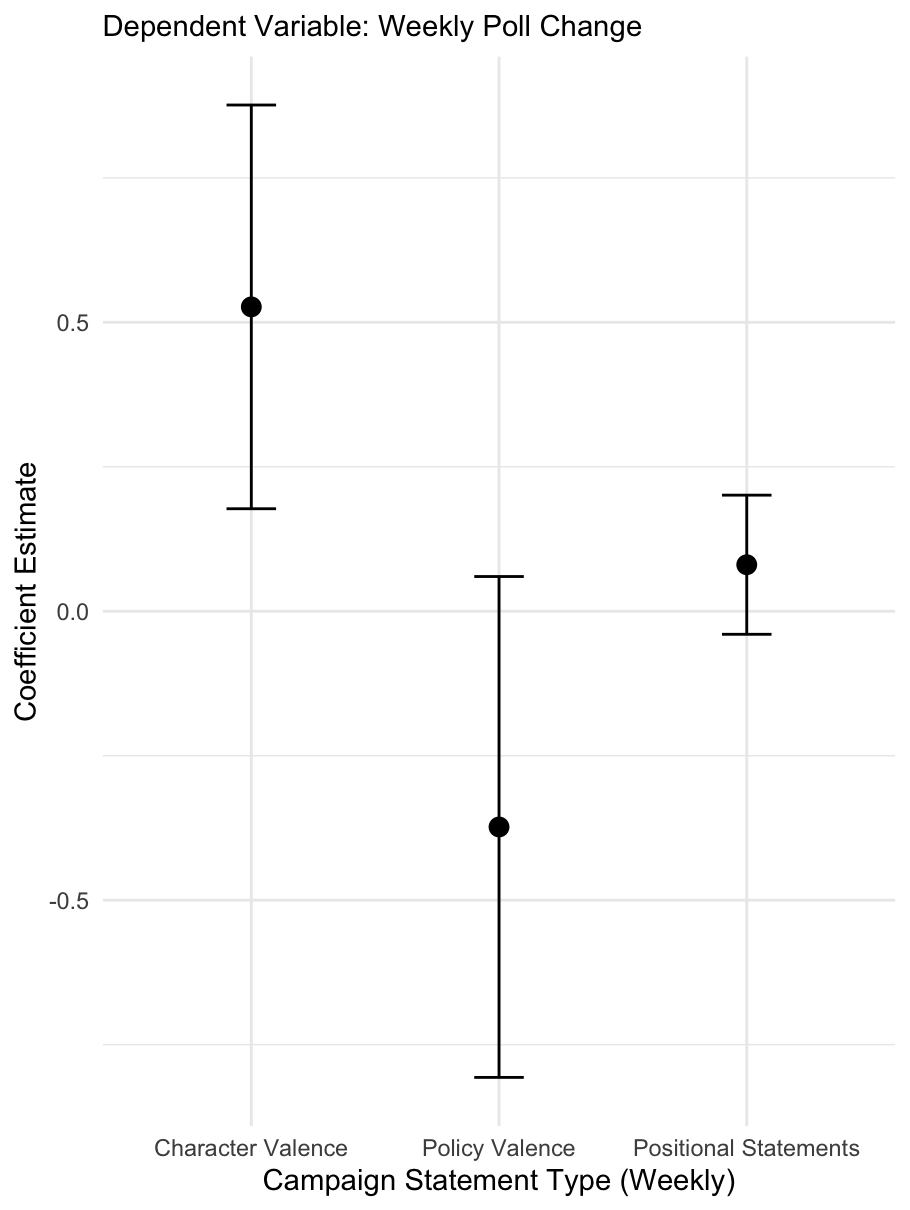
\includegraphics[width=0.7\linewidth]{images/poll_valence.png}
            \label{fig:poll_valence}
        \end{figure}
        
        \begin{table}[!htbp] \centering
            \resizebox{\linewidth}{!}{%
            \begin{tabular}{l c} 
            \hline
            \hline \\[-1.8ex]
             & \textit{$\Delta$ Poll Weekly} \\ 
            \hline \\[-1.8ex] 
            Policy Valence & $-$0.373 \\ 
            & (0.221) \\ 
            Character Valence & 0.527$^{**}$ \\ 
            & (0.178) \\ 
            Positional & 0.080 \\ 
            & (0.061) \\ 
            \hline \\[-1.8ex]
            Observations & 1,970 \\ 
            \hline
            \hline \\[-1.8ex]
            \multicolumn{2}{l}{\footnotesize \textit{Note:} Robust standard errors clustered at the party level.} \\
            \multicolumn{2}{l}{\footnotesize $^{*}$p$<$0.05; $^{**}$p$<$0.01; $^{***}$p$<$0.001} \\ 
            \end{tabular}%
            }
        \end{table}
    \end{multicols}
\end{frame}

\begin{frame}{Preliminary Results - H3}
    \begin{multicols}{2}
        \begin{figure}
            \centering
            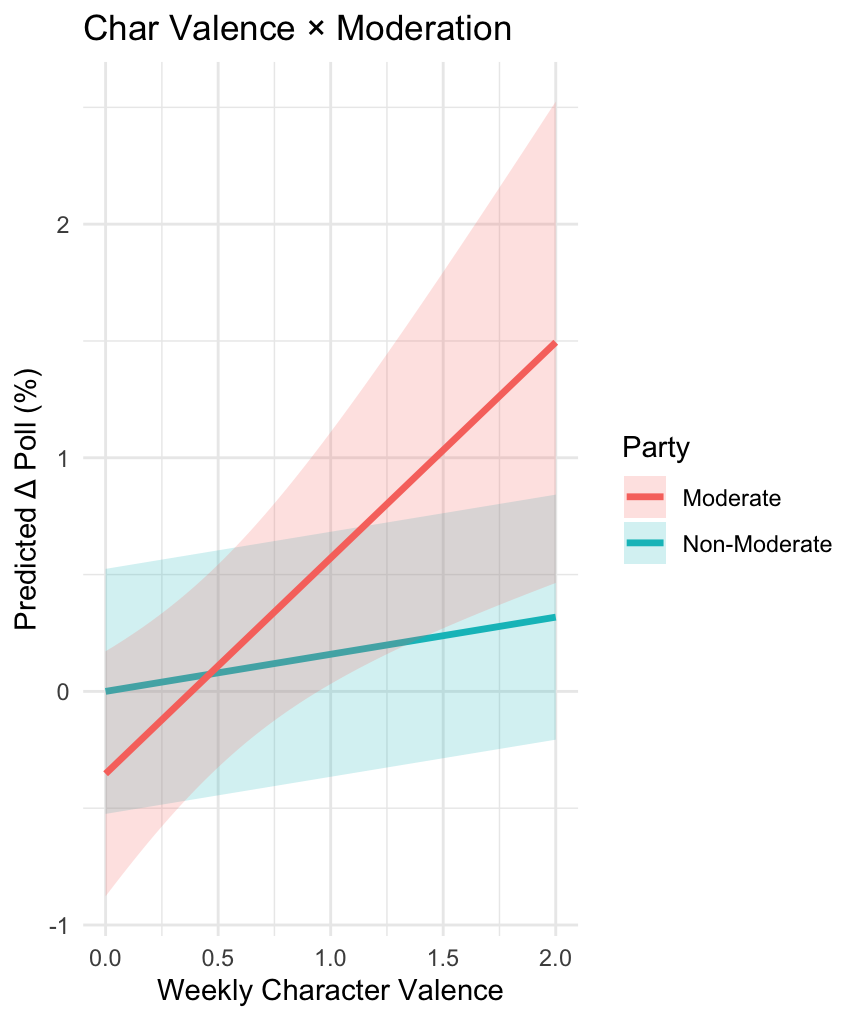
\includegraphics[width=0.8\linewidth]{images/poll_moderation.png}
            \label{fig:me_moderation}
        \end{figure}
        
\begin{table}[!htbp] \centering
\resizebox{\linewidth}{!}{%
\begin{tabular}{l c} 
\hline
\hline \\[-1.8ex]
 & \textit{$\Delta$ Poll Weekly} \\ 
\hline \\[-1.8ex] 
Character Valence & 0.159 \\ 
 & (0.268) \\ 
Moderation & $-$0.353 \\ 
 & (0.187) \\ 
Policy Valence & $-$0.566$^{**}$ \\ 
 & (0.212) \\ 
Positional & 0.118 \\ 
 & (0.072) \\ 
Character Valence × Moderation & 0.765$^{*}$ \\ 
 & (0.314) \\ 
\hline \\[-1.8ex] 
Observations & 861 \\
\hline
\hline \\[-1.8ex]
\multicolumn{2}{l}{\footnotesize  \textit{Note:} Robust standard errors clustered at the party level.} \\
\multicolumn{2}{l}{\footnotesize $^{*}$p$<$0.05; $^{**}$p$<$0.01; $^{***}$p$<$0.001} \\ 
\end{tabular}%
}
\end{table}
    \end{multicols}
\end{frame}

%%% PAPER 2
\begin{frame}{Economic Performance Indicators and Strategic Valence Choices}
    \textbf{Main Research Questions} \vspace{0.1cm}
    \begin{itemize}
        \item \textbf{RQ1:} How do governing parties adjust their emphasis on valence traits in response to economic indicators?\vspace{0.1cm}
        \item \textbf{RQ2:} How do opposition parties adjust their communication strategies around economic issues in response to economic indicators?
    \end{itemize}
    \vspace{0.4cm}
    \textbf{Theoretical Expectations} \customcite{Greene2015}\vspace{0.1cm}
\begin{itemize}
    \item \textbf{H1:} Governing parties emphasize valence traits when economic performance indicators are positive\vspace{0.1cm}
    \item \textbf{H2:} Opposition parties emphasize valence traits when economic performance indicators are negative\vspace{0.1cm}
    \item \textbf{H3:} Opposition parties highlight positional issues (e.g. redistribution) to challenge the incumbent\vspace{0.1cm}
    \item \textbf{H4:} Parties select issue emphasis strategically, based on whether they can claim credit or shift blame
\end{itemize}   
    \end{frame}

\begin{frame}{Research Design}
    \textbf{Data:} \vspace{0.1cm}
    \begin{itemize}
        \item Parliamentary debates: ParlaMint \customcite{erjavec2023parlamint}, ParlSpeech \customcite{rauh2020parlspeech} \vspace{0.1cm}
        \item Economic performance indicators (e.g. GDP growth, unemployment rates)
    \end{itemize}
    \vspace{0.3cm}
    
    \textbf{Methodology:} \vspace{0.1cm}
    \begin{itemize}
        \item Use a Natural Language Inference (NLI) approach to classify debates:\vspace{0.1cm}
        \begin{itemize}
            \item "Economic-Related" valence traits: competence in managing the economy, effective governance, and leadership during economic crises \vspace{0.1cm}
            \item Positional issues: specific policy stances on economic matters \vspace{0.1cm}
        \end{itemize}
        \item Fine-tune an NLI classifier, such as Political DEBATE \customcite{burnham2024political} \vspace{0.1cm}
        \item For political text classification, smaller fine-tuned LLMs consistently outperform larger zero-shot prompted models \customcite{bucher2024finetunedsmallllmsstill} \vspace{0.1cm}
        \item Analyze how governing parties emphasize economic valence traits in response to positive economic indicators \vspace{0.1cm}
        \item Examine how opposition parties shift focus to positional issues under similar conditions
    \end{itemize}
    \vspace{0.3cm}
\end{frame}

\begin{frame}{Conclusions and Next Steps}
    \textbf{Political Scandals and Voter Evaluations}
    \begin{itemize}
        \item Reflect on the wording of the attributes, complete the pre-registration
        \item Validate the tones using SpeechBrain \customcite{speechbrain} trained on IEMOCAP
        \item Compare the advantages of LLM-generated vs. manually written debate scripts to capture natural political discourse
    \end{itemize}
    \vspace{0.2cm}
    \textbf{Electoral Campaigns and Valence}
    \begin{itemize}
        \item Expand polling data coverage for additional elections and countries
        \item Conduct potential robustness checks to ensure the validity of results (e.g. Autoregressive Models, More controls)
        \item Test the role of policy moderation/change 
    \end{itemize}
    \vspace{0.2cm}
    \textbf{Economic Performance and Strategic Valence}
    \begin{itemize}
        \item Develop hypotheses for the Natural Language Inference (NLI) classifier
        \item Construct a fine-tuning dataset for economic valence traits and positional issues
        \item Explore classical topic modeling approaches and LLM-based topic classification
    \end{itemize}
    \end{frame}

\begin{frame}[plain]
\centering
\vspace{2cm}
\textbf{\large Thank You for Your Attention!} \\ [0.2cm] 
\texttt{stefano.sangiovanni@unimi.it} \\[3cm]

% Social Media Links with Icons
\faGithub\ \href{https://github.com/ste-sangiovanni}{ste-sangiovanni} \\[0.1cm]
\faTwitter\ @stesangio \\ 

\includegraphics[width=0.03\textwidth]{images/Bluesky_logo_(black).svg.png} @stesangio.bsky.social
\vspace{0.2cm}
\end{frame}

\begin{frame}[plain, allowframebreaks, c]
    \centering
    \vspace*{2em}
    \printbibliography
\end{frame}

\begin{frame}{Appendix 1.1 - Power Analysis - 0.05 es}
    \begin{figure}
        \centering
        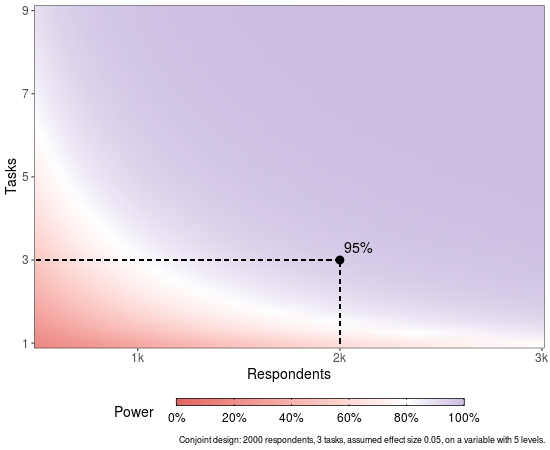
\includegraphics[width=0.6\linewidth]{images/pa_3task.png}
        \label{fig:appendix1}
    \end{figure}
\end{frame}

\begin{frame}{Appendix 1.2 - Power Analysis - 0.04 es}
    \begin{figure}
        \centering
        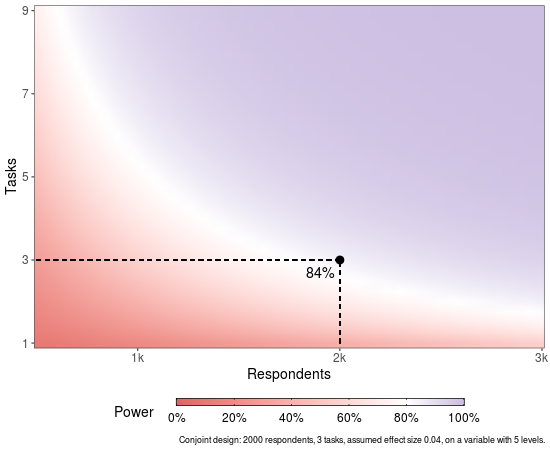
\includegraphics[width=0.6\linewidth]{images/pa_3task_0.4effect.png}
        \label{fig:appendix2}
    \end{figure}    
\end{frame}

% \begin{frame}{Appendix 2.1 - Main Theoretical Expectations - Conjoint Experiment}
% \begin{itemize}
%     \item \textbf{H1a:} Respondents will prefer candidates with no scandals over those with scandals, regardless of other candidate attributes. \vspace{0.2cm}
%     \item \textbf{H1b:} Financial scandals will have a stronger negative impact on respondent preferences than personal scandals. \vspace{0.2cm}
%     \item \textbf{H1c:} Positive valence will mitigate the negative impact of scandals on respondent preferences, with higher positive valence reducing the severity of both financial and personal scandals. \vspace{0.2cm}
%     \item \textbf{H1d:} Respondents will be more forgiving of candidates with the same party affiliation when the candidate has a scandal. \vspace{0.2cm}
%     \item \textbf{H1e:} Respondents will prefer candidates whose policy positions align more closely with their own, even if the candidate has a scandal. \vspace{0.2cm}
% \end{itemize}
% \end{frame}

% \begin{frame}{Appendix 2.2 - Main Theoretical Expectations - Conjoint Experiment}
% \textbf{Gender and Standards of Evaluation:}
% \begin{itemize}
%     \item \textbf{H2a:} Female candidates will be held to higher standards regarding scandals than male candidates, with respondents showing a stronger negative response to scandals involving female candidates. \vspace{0.2cm}
%     \item \textbf{H2b:} Female candidates with scandals will suffer a greater decline in respondent support compared to male candidates with similar scandals. \vspace{0.2cm}
% \end{itemize}

% \textbf{Policy vs. Scandal Mitigation:}
% \begin{itemize}
%     \item \textbf{H3a:} A candidate’s policy position will be more influential than their scandal history when respondents share the same political alignment as the candidate. \vspace{0.2cm}
%     \item \textbf{H3b:} The negative impact of a scandal will be diminished if the candidate’s policy position aligns closely with the respondent's preferences, particularly for co-partisan candidates. \vspace{0.2cm}
% \end{itemize}
% \end{frame}


\begin{frame}{Appendix 2.1 - Prompt Example}
        \begin{figure}
        \centering
        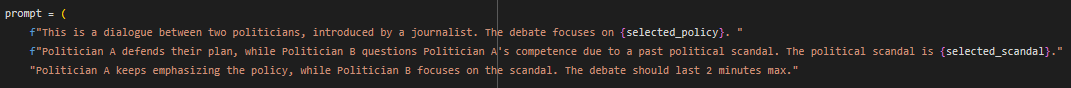
\includegraphics[width=\linewidth]{images/Prompt 1.png}
        \label{fig:appendix_prompt1}
    \end{figure}  
\end{frame}

\begin{frame}{Appendix 2.2 - Prompt Example}
        \begin{figure}
        \centering
        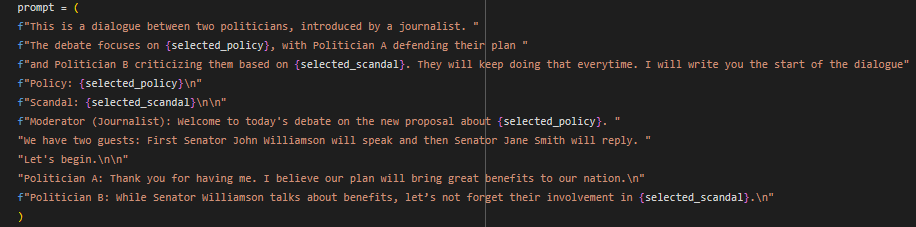
\includegraphics[width=\linewidth]{images/prompt 2.png}
        \label{fig:appendix_prompt2}
    \end{figure}  
\end{frame}

\begin{frame}{Appendix 3.1 - Full Profile Table}
\begin{table}[!h]
\centering
\resizebox{\textwidth}{!}{%
\begin{tabular}{|c||c|}
\hline
\textbf{Attributes}                 & \textbf{Levels}                                                                                                    \\ \hline
\textbf{Gender}                     & \begin{tabular}[c]{@{}c@{}}Male \\[2pt] Female\end{tabular}                                                              \\ \hline
\textbf{Party Affiliation}          & \begin{tabular}[c]{@{}c@{}}Right-Wing \\[2pt] Left-Wing\end{tabular}                                      \\ \hline
\textbf{Incumbency Status}          & \begin{tabular}[c]{@{}c@{}}Incumbent \\[2pt] Opposition\end{tabular}                                      \\ \hline
\textbf{Position on Immigration}    & \begin{tabular}[c]{@{}c@{}}Implement strict border controls and reduce immigration \\[2pt]
Promote inclusive immigration policies and increase quotas for asylum seekers
\end{tabular}       \\ \hline
\textbf{Position on Economic Policies} & \begin{tabular}[c]{@{}c@{}}Advocates for tax reductions, market deregulation and business-friendly policies \\[2pt]
Supports stronger market regulations, higher corporate taxation and expanded welfare programs
\end{tabular} \\ \hline
\textbf{Political Scandal} &  \begin{tabular}[c]{@{}c@{}}No scandal \\[2pt] Investigated for unwanted sexual conduct towards staff members \\[2pt] Falsification of credentials on curriculum vitae \\[2pt] Investigated for corruption \\[2pt] Participated in a violent anti-government protest while underage

 \end{tabular} \\ \hline
\textbf{Positive Valence} &  \begin{tabular}[c]{@{}c@{}}No positive valence \\[2pt] Had 95\% of campaign statements certified as accurate by an independent fact checker \\[2pt] Led public-private partnership preventing layoffs during local economic downturn \\[2pt] Successfully rallied party support for innovative policy agenda, turning initial 30\% backing into 90\% consensus \\[2pt] Voted with party positions on 93\% of legislative votes
 \end{tabular} \\ \hline
\end{tabular}%
}
\end{table}
\end{frame}

\begin{frame}{Appendix 3.2 - Valence vs Valence}
    \begin{table}[!h]
\centering
\resizebox{\textwidth}{!}{%
\begin{tabular}{|c||c|}
\hline
\textbf{Attributes}                 & \textbf{Levels}                                                                                                    \\ \hline
\textbf{Political Scandal} &  \begin{tabular}[c]{@{}c@{}}No scandal \\[2pt] Investigated for unwanted sexual conduct towards staff members \\[2pt] Falsification of credentials on curriculum vitae \\[2pt] Investigated for appropriation of illegal funding \\[2pt] Participated in a violent anti-government protest while underage

 \end{tabular} \\ \hline
\textbf{Positive Valence} &  \begin{tabular}[c]{@{}c@{}}No positive valence \\[2pt] Received an award for championing workplace equity and inclusion from the National Diversity \& Inclusion Association
 \\[2pt]He had 95\% of campaign statements certified as accurate by an independent fact checker
\\[2pt] Led a public-private partnership that prevented layoffs during a local economic downturn
 \\[2pt] Received a national award for community service while underage

 \end{tabular} \\ \hline
\end{tabular}%
}
\end{table}
\end{frame}

\begin{frame}{Appendix 4.1 - Literature Gaps in Political Scandal Research}
    \begin{itemize}
        \item Limited focus on types of scandals beyond corruption, reducing generalizability \customcite{kumlin2012scandal} \vspace{0.3cm}
        \item Insufficient research on voters' reactions to different types of scandals \vspace{0.3cm}
        \item Lack of systematic comparisons across various contexts (moral values are country dependent), scandal types and valence informations \customcite{kumlin2012scandal} \vspace{0.3cm}
        \item Effects of different scandal types on electoral behavior in polarized contexts remain poorly understood \customcites{puglisi2011, darr2019collision, Rottinghaus_2023} \vspace{0.3cm} 
    \end{itemize}
\end{frame}

\begin{frame}{Appendix 4.2 - Experiment Data Analysis Approach}
    \begin{itemize}
\item \textbf{AMCE:} The average effect of varying one attributes of a profile on the probability that that profile will be chosen by a respondent \customcite{BansakEtAl2022}\vspace{0.3cm} 
\item \textbf{Marginal Means:} An alternative estimator that does not rely on reference categories and is gaining preference in recent research \customcite{Casiraghi} \vspace{0.3cm} 
        \item \textbf{Exploratory Analyses:}  
        \begin{itemize}
            \item \textbf{ACIEs:} Examining how the impact of one attribute (e.g. party affiliation) depends on another (e.g. scandal) \vspace{0.2cm}  
            \item \textbf{Subgroup analyses:} Preference heterogeneity across respondent characteristics \customcite{Leeper_Hobolt_Tilley_2020} \vspace{0.2cm} 
        \end{itemize}
    \end{itemize}
\end{frame}

\begin{frame}{Appendix 5 - Valence and Polls Dataset example}
    \begin{table}[!htbp] \centering 
        \caption{Salection of Valence/Polls Dataset} 
        \label{tab:uk_election_preview} 
      \small 
      \begin{tabular}{cccccccc} 
      \\[-1.8ex]\hline 
      \hline \\[-1.8ex] 
      country & election\_year & date & party & char.val & pol.val & pos & poll\_perc \\ 
      \hline \\[-1.8ex] 
      UK & 2005 & 2005-04-05 & Conservative Party & 0 & 0 & 3 & 35.25 \\ 
      UK & 2005 & 2005-04-05 & Labour Party & 2 & 1 & 5 & 36 \\ 
      UK & 2005 & 2005-04-05 & Liberal Democratic Party & 1 & 2 & 1 & 20.5 \\ 
      UK & 2005 & 2005-04-06 & Conservative Party & 2 & 1 & 6 & 36 \\ 
      UK & 2005 & 2005-04-06 & Labour Party & 4 & 4 & 16 & 36 \\ 
      UK & 2005 & 2005-04-06 & Liberal Democratic Party & 1 & 0 & 3 & 21 \\ 
      \hline \\[-1.8ex] 
      \multicolumn{8}{l}{Sample of dataset.} \\ 
      \end{tabular} 
      \end{table} 
\end{frame}

\begin{frame}{Appendix 5 - Valence and Polls}
    \begin{figure}
        \centering
        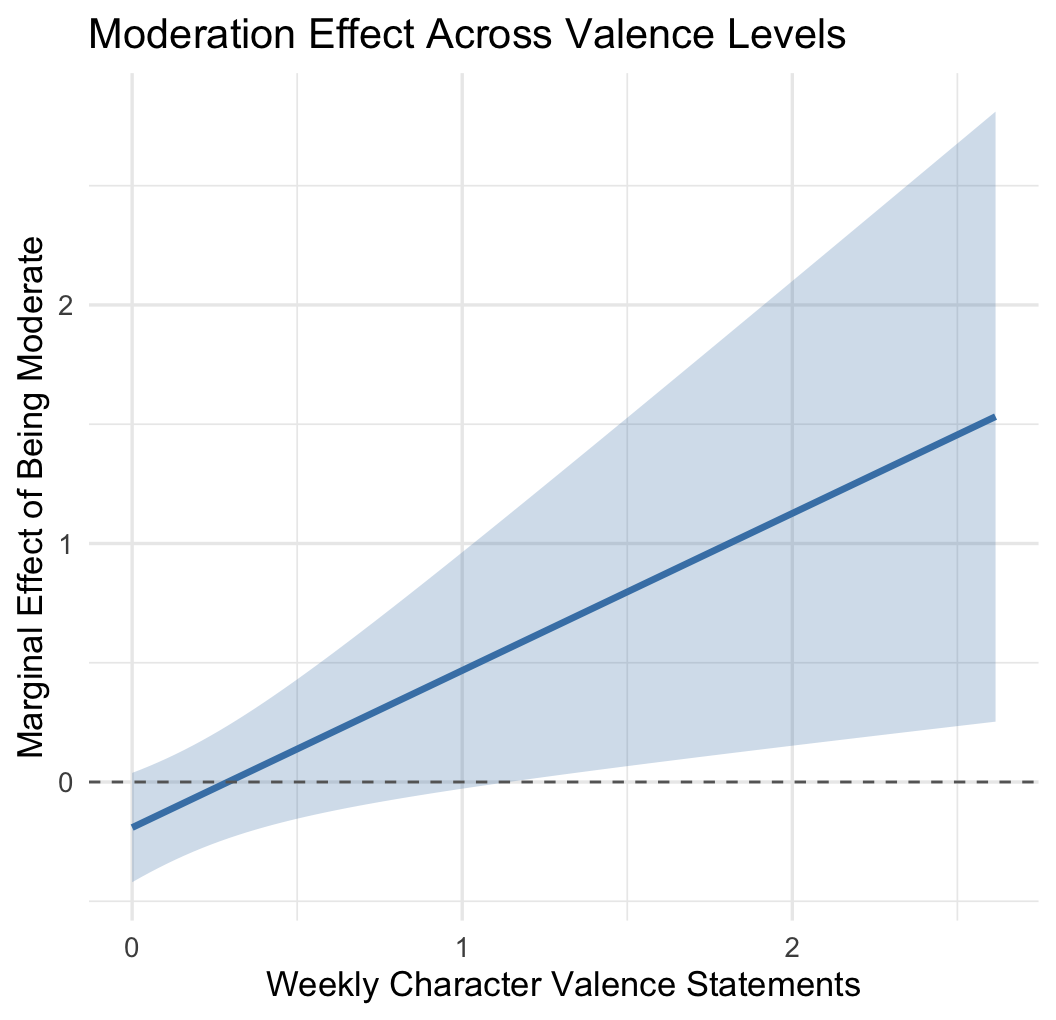
\includegraphics[width=0.4\textwidth]{images/me_moderation.png}
        \label{fig:poll_moderation2}
    \end{figure}
\end{frame}


\end{document}
